\chapter{Results}
\label{chap:Results}


\begin{figure}[H]
    \center
    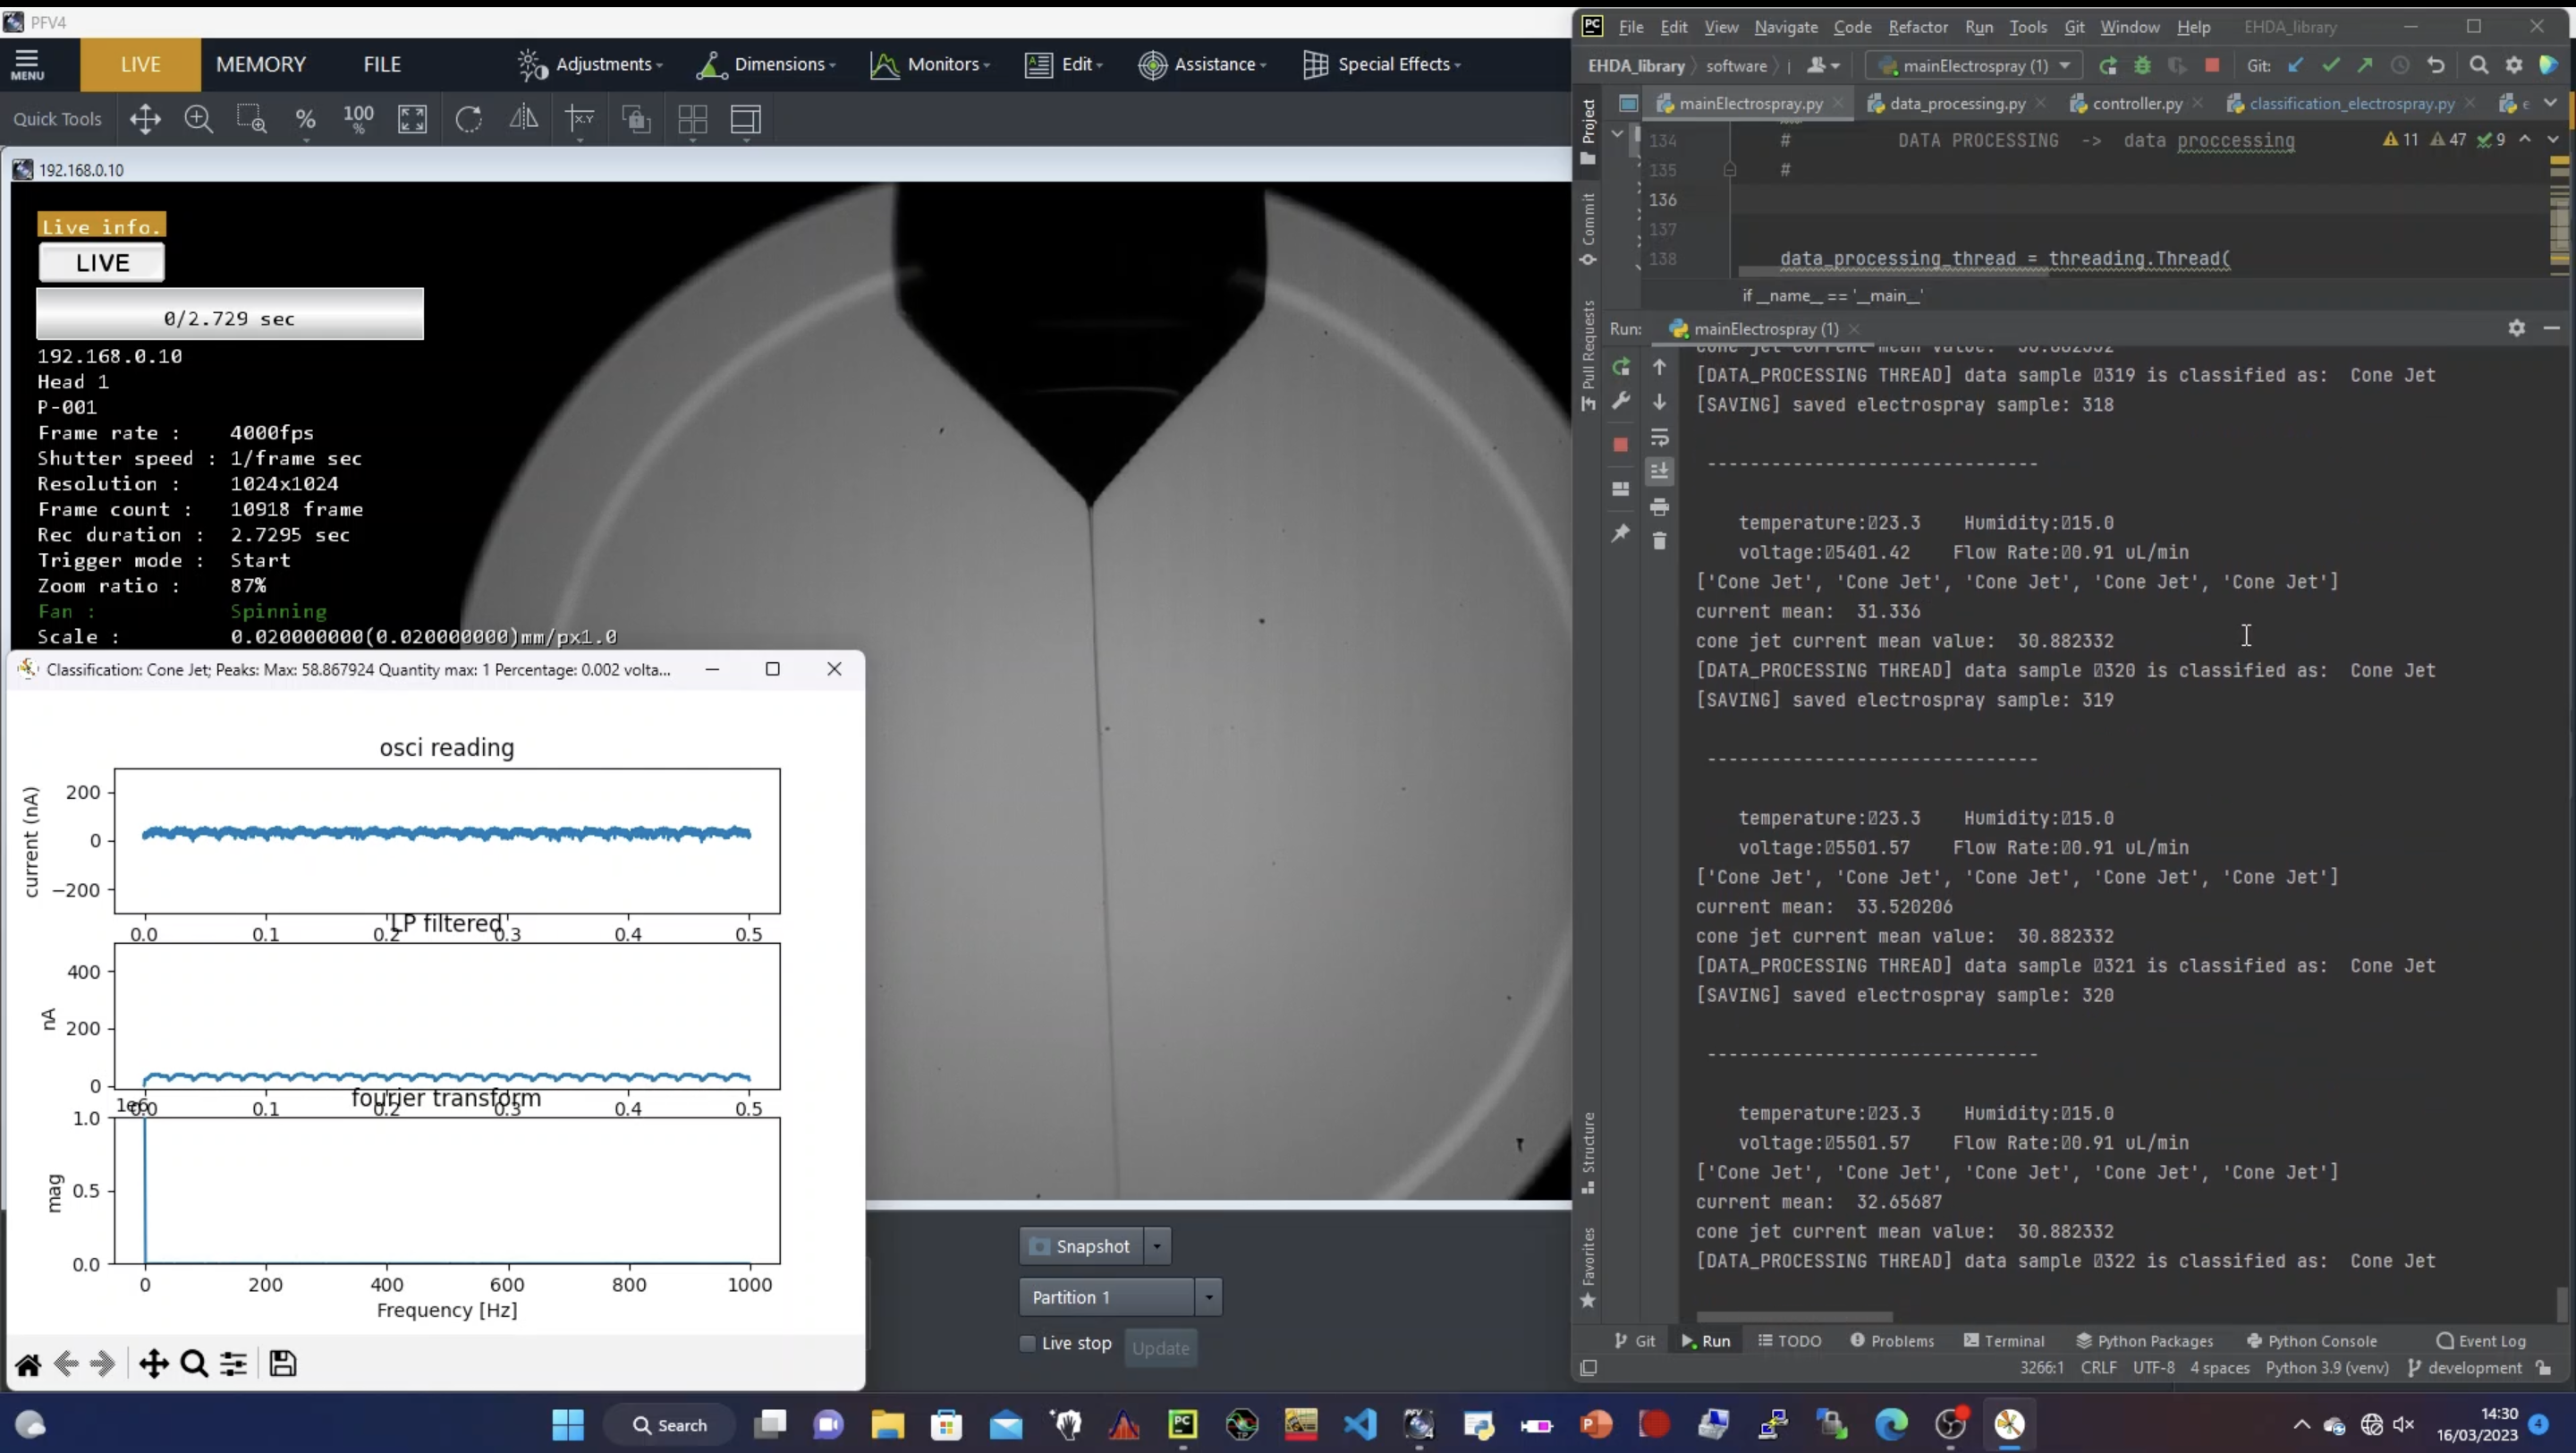
\includegraphics[width=17cm]{Figuras/19:03/axs1.png}
    \caption{Printscreen of the window shows user interface during the experiment.
        We can see the image generated by the camera in the background.
        The routine code running in pycharm software on the right side.
        And also real time signal plottings of the current data on the left side.}
\end{figure}


\begin{figure}[H]
    \centering
    \resizebox{170mm}{!}{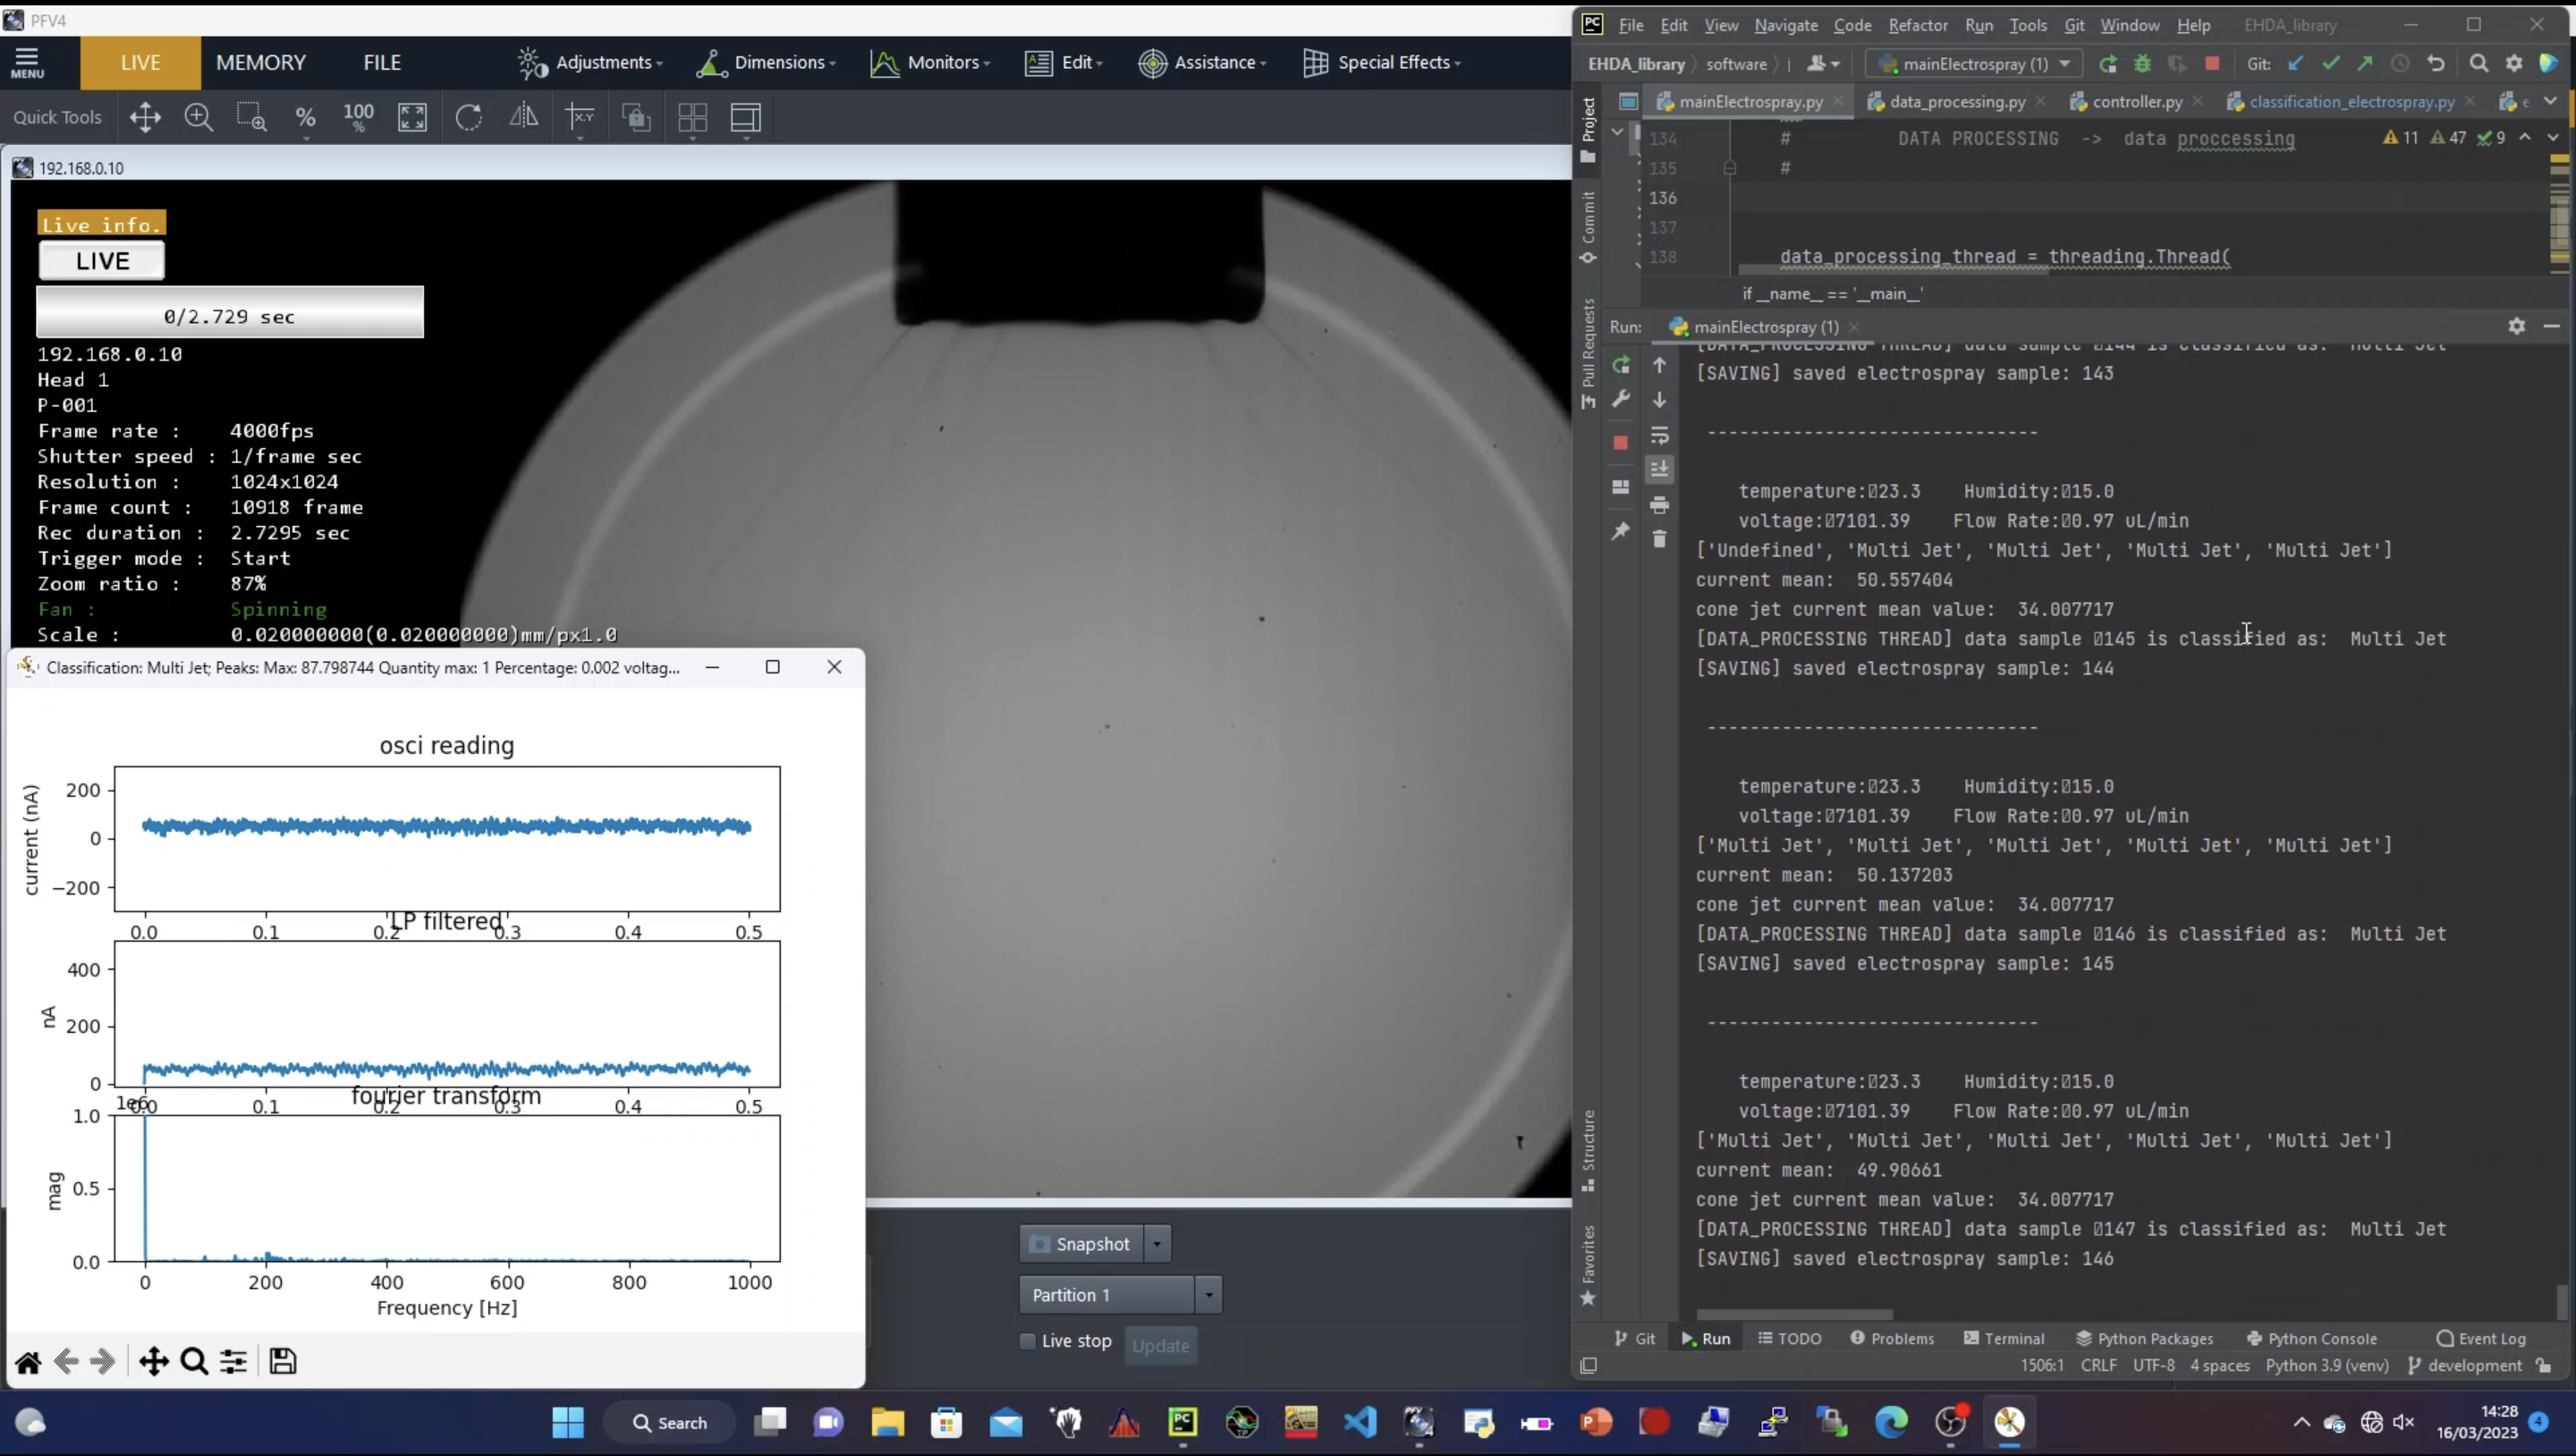
\includegraphics{Figuras/19:03/axs2.png}}
    \caption{Printscreen during an experiment. At this moment we are in Multi Jet spraying mode. At the left we can see the current signal has a smoth and constant curve. We can also see the automatic classification at the right side.}
    \label{fig:multi_class_exp}
\end{figure}


\section{Classification}
\label{sec:classification_results}

The results of the classification using the statistical values are illustrated in figures \ref{fig:step_voltage}, \ref{fig:raw_data} and \ref{fig:class_step_data}.


\begin{figure}[H]
    \center
    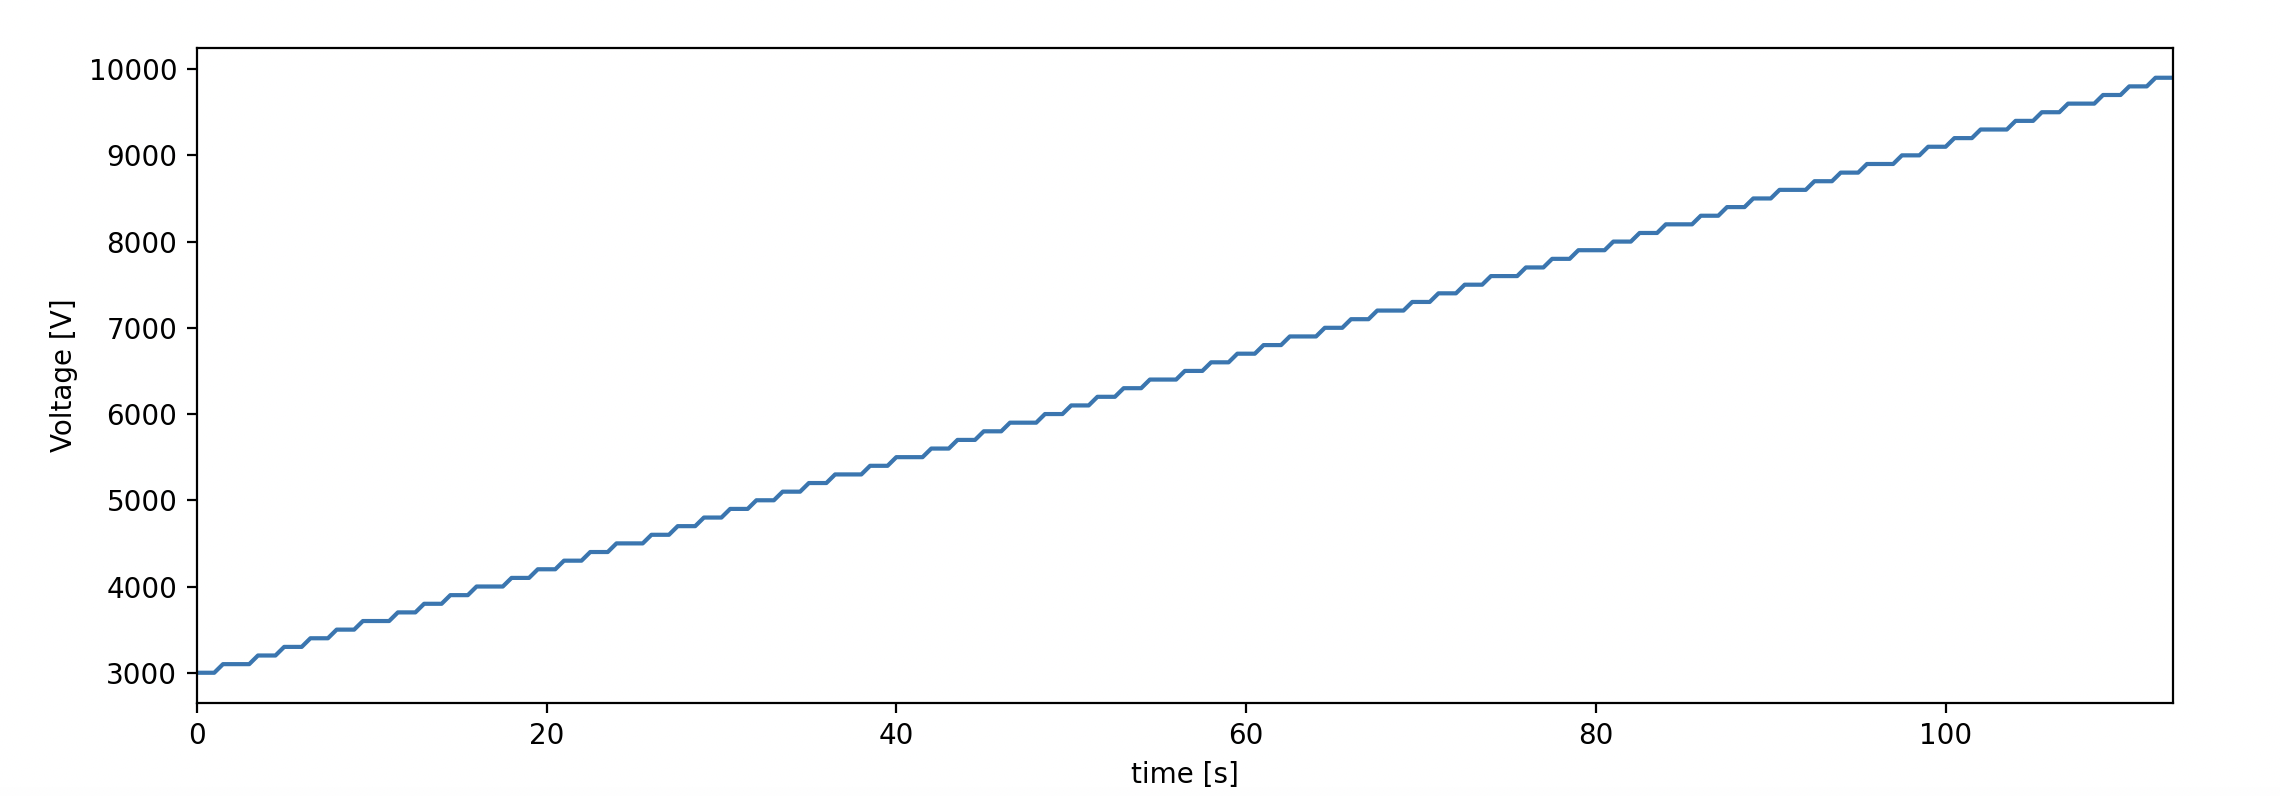
\includegraphics[width=12cm]{Figuras/19:03/voltage_step.png}
    \caption{Input voltage step graph. The range is between 3K-10K Volts. Step size of 50V and steo time of 5 seconds.}
    \label{fig:step_voltage}
\end{figure}


\begin{figure}[H]
    \center
    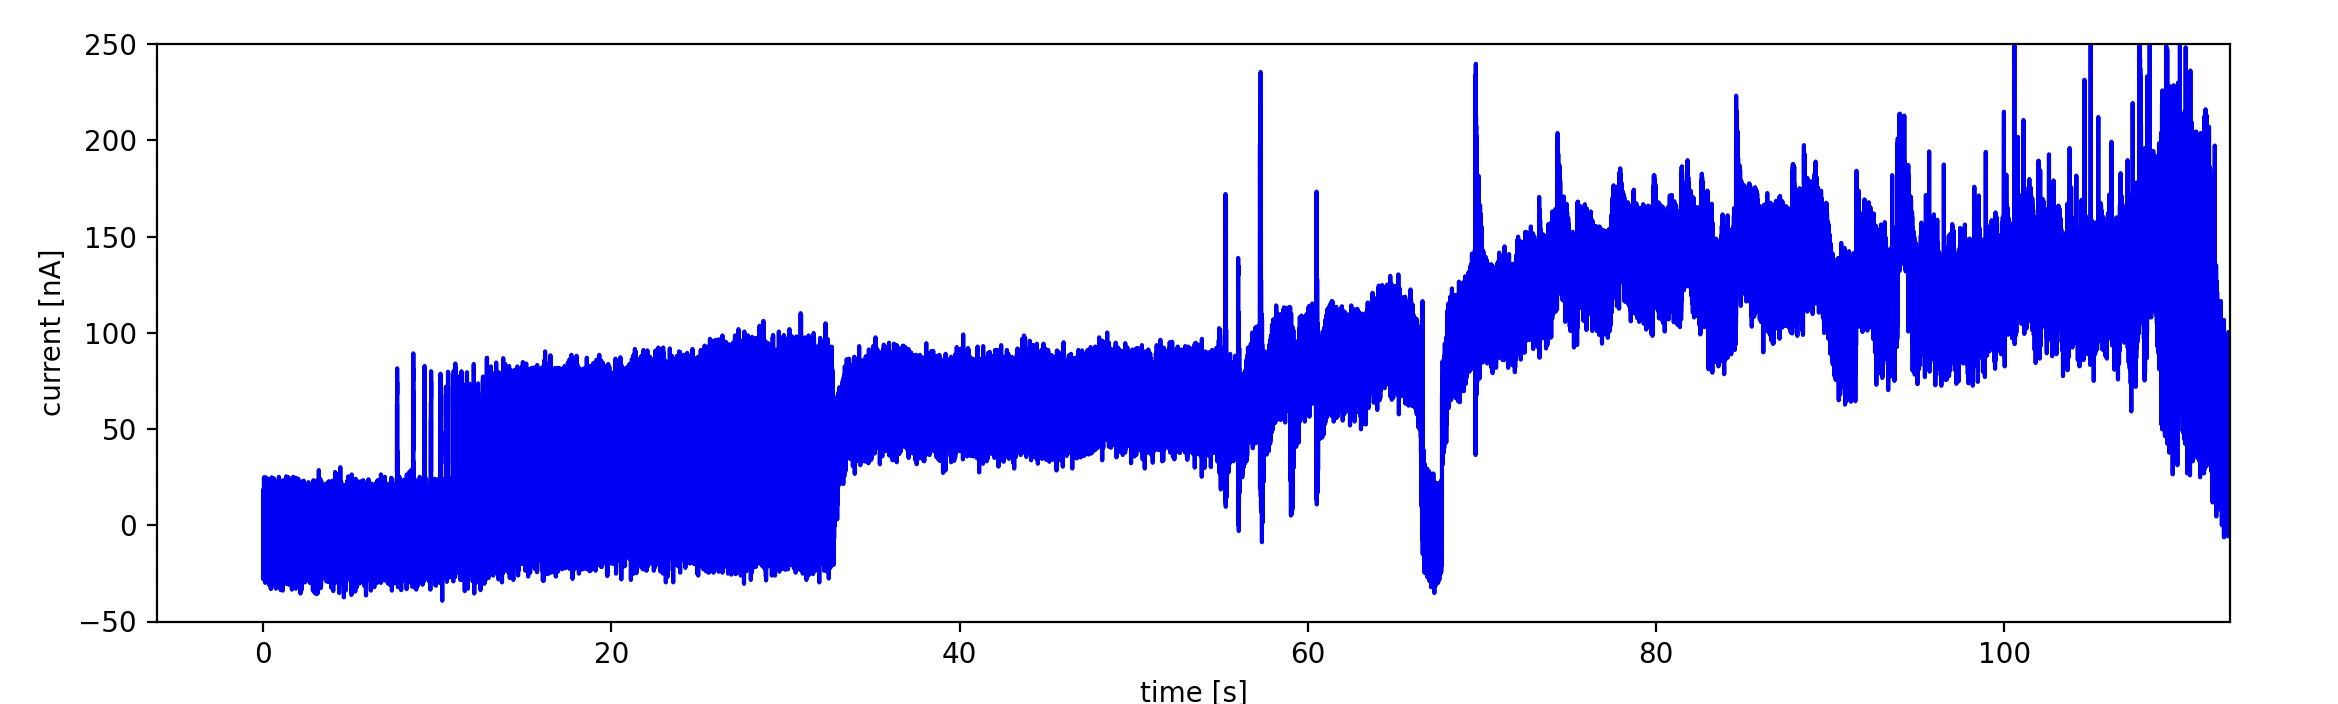
\includegraphics[width=12cm]{Figuras/19:03/raw-data-example.png}
    \caption{Output raw data collected in the voltage range experiment showed in \ref{fig:step_voltage}. The sampling rate of the oscilloscope is 10KHz. This graph has 1.5 Million data points.}
    \label{fig:raw_data}
\end{figure}

Notice that is even possible to a visual classification. The Dripping mode has a current mean of 0V. The Intermittent state has a high variation of values that can be seen by the thickness of the graph. The Cone jet is a thiner graph because the signal is more constant. The Multi Jet is the same as Cone jet graph but with a higher mean value than cone Jet.


\begin{figure}[H]
    \center
    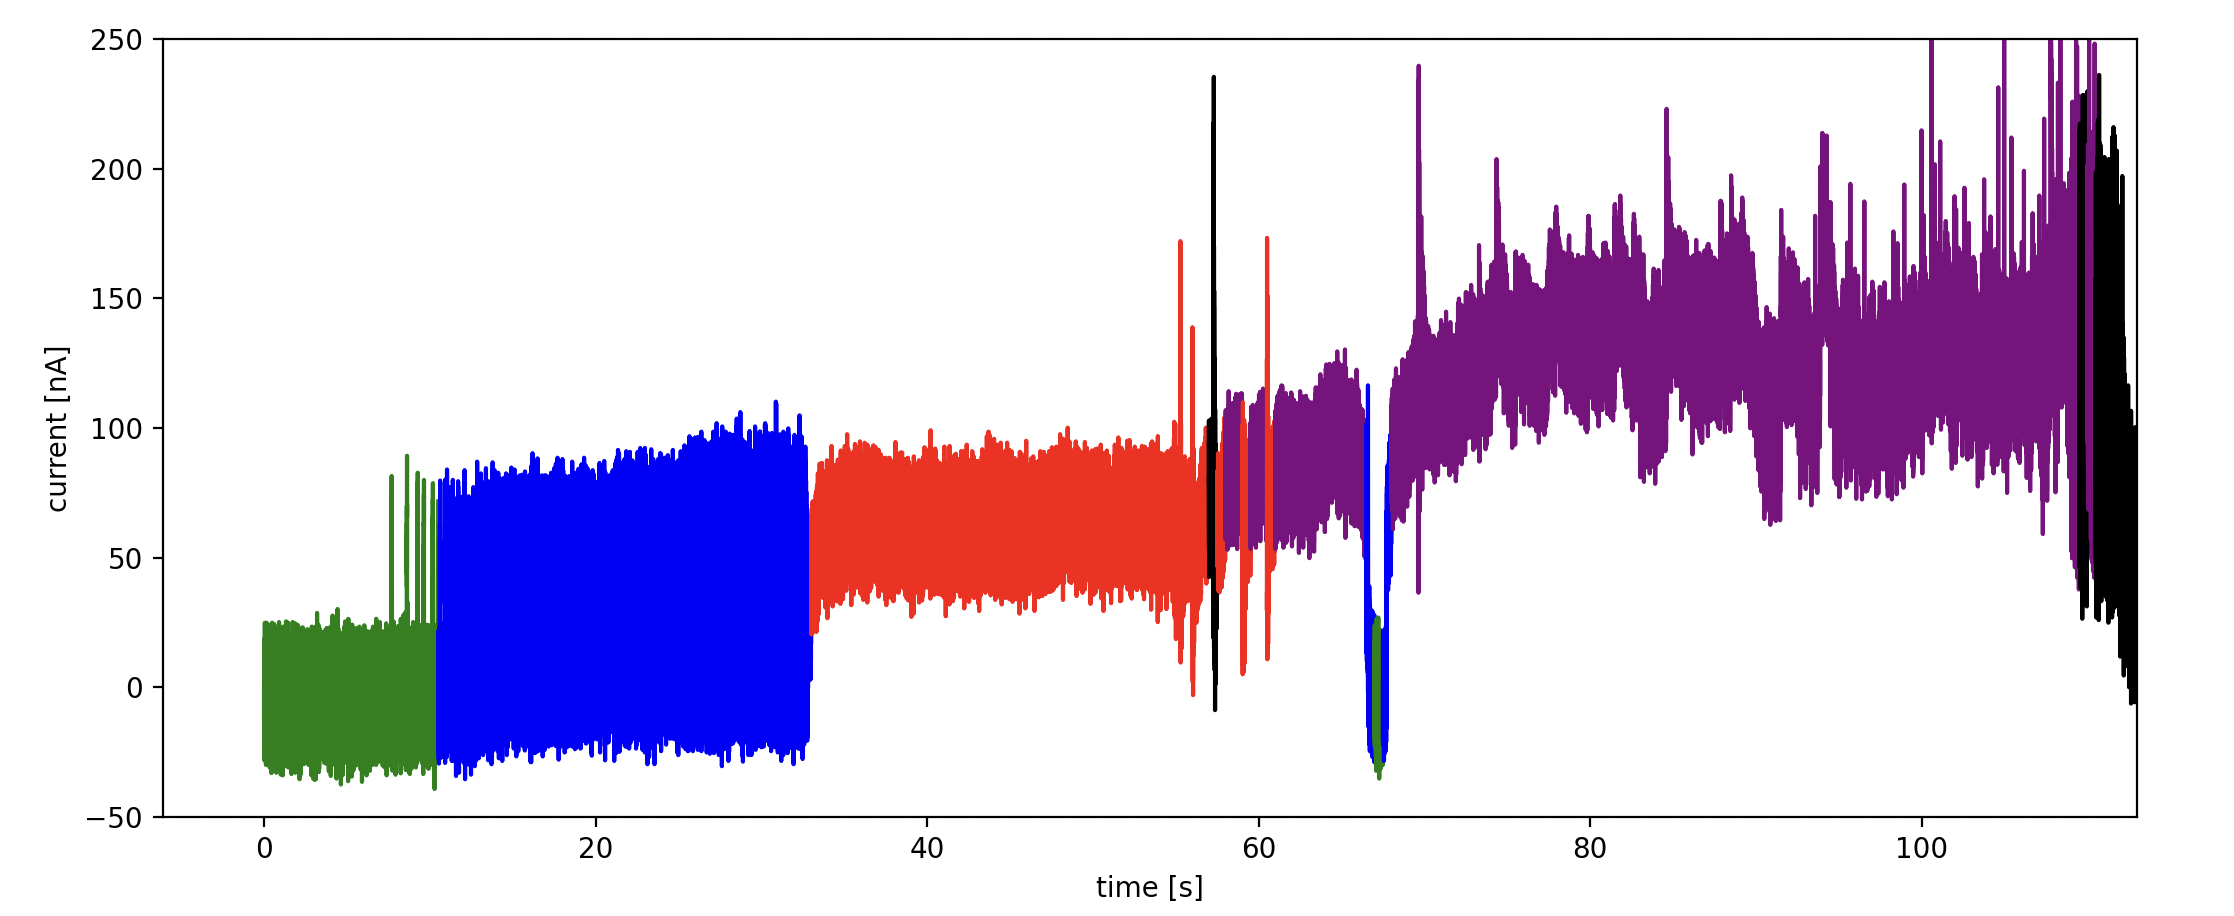
\includegraphics[width=12cm]{Figuras/19:03/classified-data-example.png}
    \caption{The same graph as \ref{fig:raw_data} but after the classification procedure. The colours are green: Dripping, Blue: Intermittent, Red: Cone Jet, Purple: Multi Jet and Black: Undefined.}
    \label{fig:class_step_data}
\end{figure}


\section{Map Sequence}
\label{sec:map_results}



    \subsection{Manual experiments}


    For better understand the effects of both voltage and flowrate in the spraying dinamycs manual experiments were made.
    Also in order to find the stability region of cone jet mode for the liquid and setup used.

    \begin{figure}[H]
        \center
        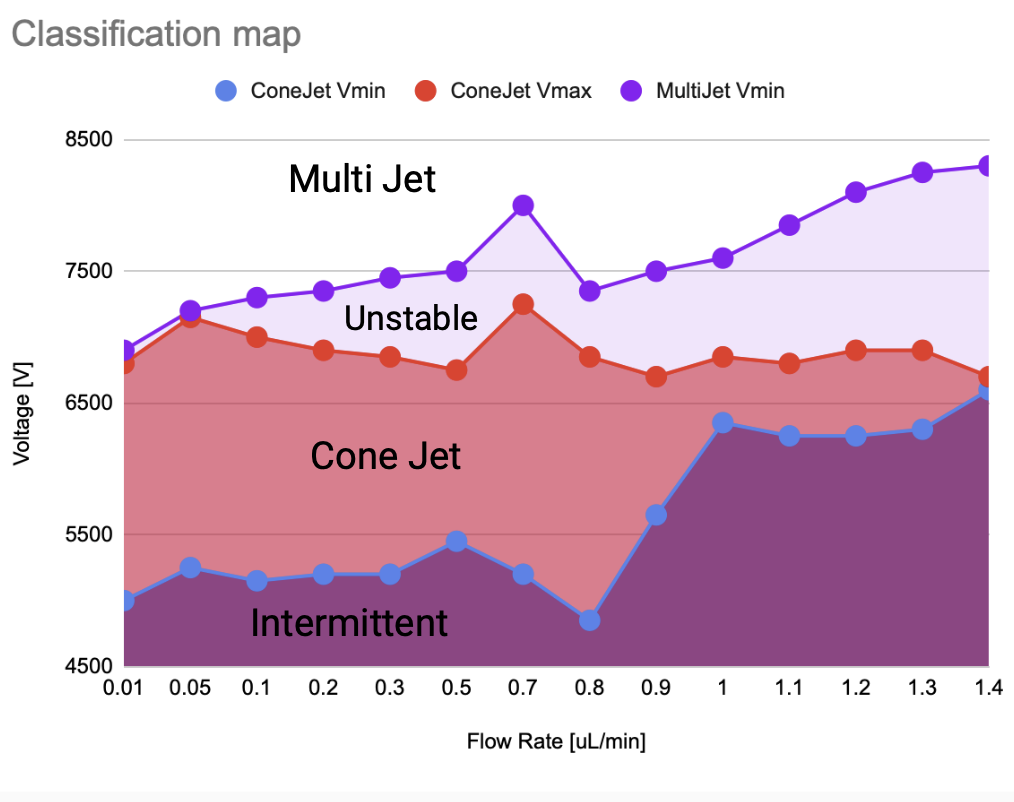
\includegraphics[width=12cm]{Figuras/regions.png}
        \caption{ exp-26-01-2 (V x Q)}
    \end{figure}


    \subsection{Manual x Automatic Cone Jet stability island maps}

        For validation of the automatic system and classification some experiments were made having both manual and automatic data collecting.



        In Figure 14 we can see a result of the map generated by the automatic classification in this experiment.

        \begin{figure}[H]
            \center
            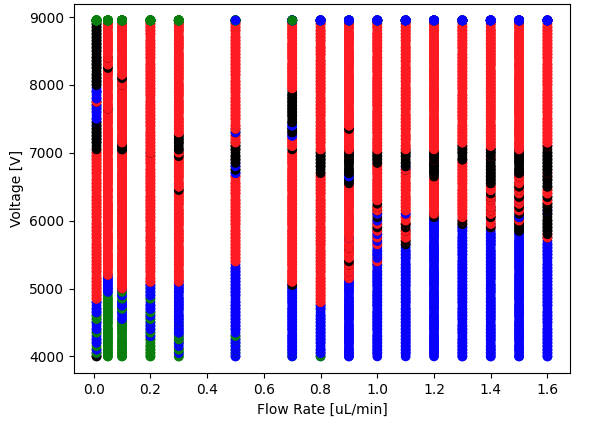
\includegraphics[width=10cm]{Figuras/report3/map-exp-26-01.png}
            \caption{ exp-26-01-23 }
        \end{figure}

        Figures 15 and 16 shows that we could achieve a stable cone jet region map with similar shape and values in both manual and automatic classification of the same experiment.

        \begin{multicols}{2}


            \begin{figure}[H]
                \center
                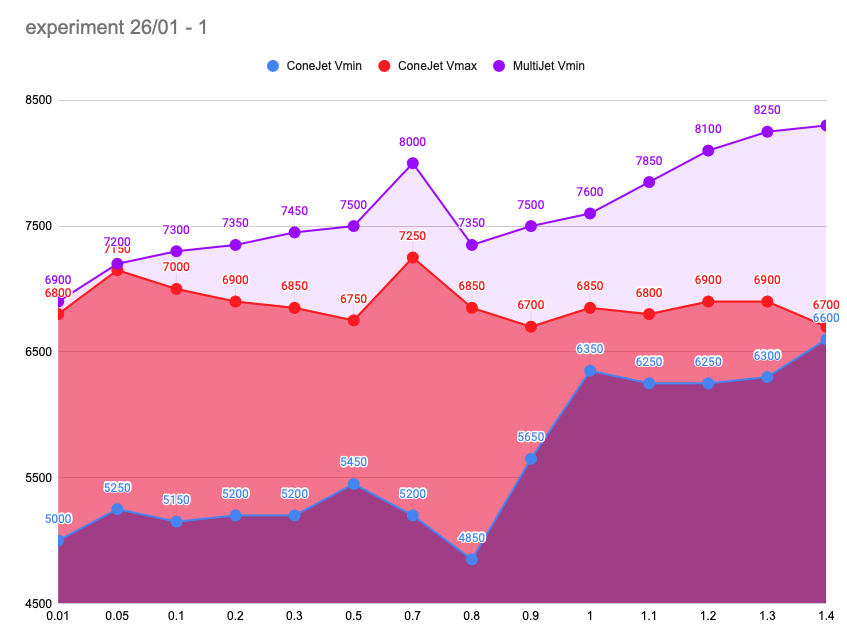
\includegraphics[width=9cm]{Figuras/report3/manual-mapping.png}
                \caption{ exp-26-01 manual classification}
            \end{figure}

            \begin{figure}[H]
                \center
                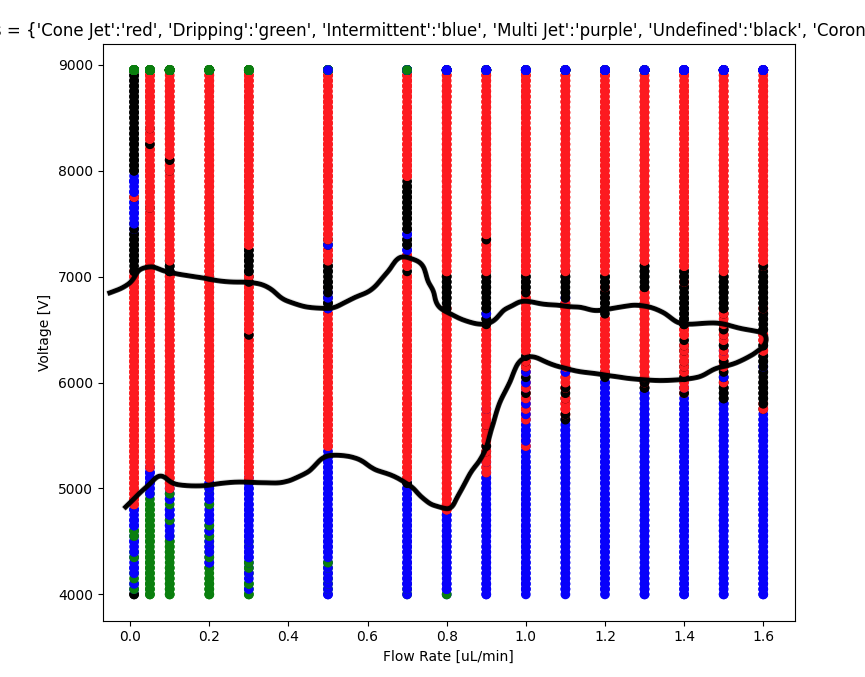
\includegraphics[width=9cm]{Figuras/report3/map4-stabilityIsland.png}
                \caption{ exp-26-01 automatic classification}
            \end{figure}

        \end{multicols}

        Figures 15 and 16 shows that we could achieve a stable cone jet region map with similar shape and values in both manual and automatic classification of the same experiment.


        \begin{multicols}{2}


            \begin{figure}[H]
                \center
                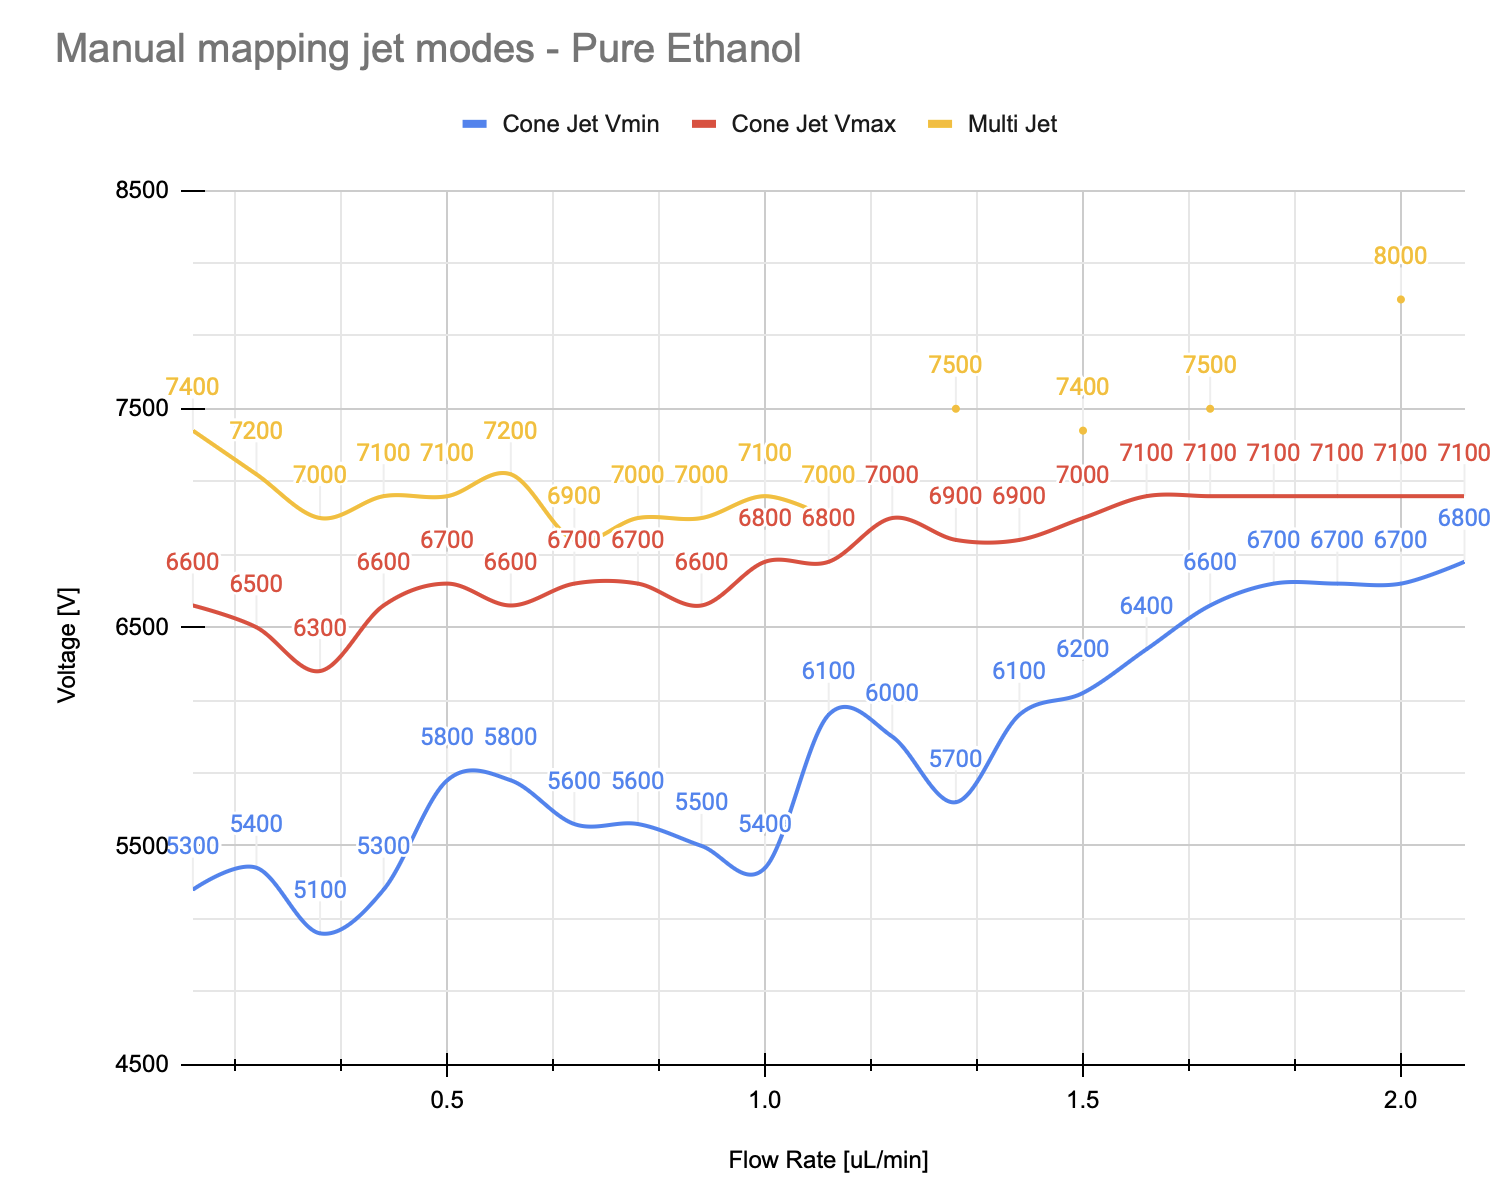
\includegraphics[width=7cm]{Figuras/report4/map7-manual.png}
                \caption{ exp-26-01 manual classification}
            \end{figure}

            \begin{figure}[H]
                \center
                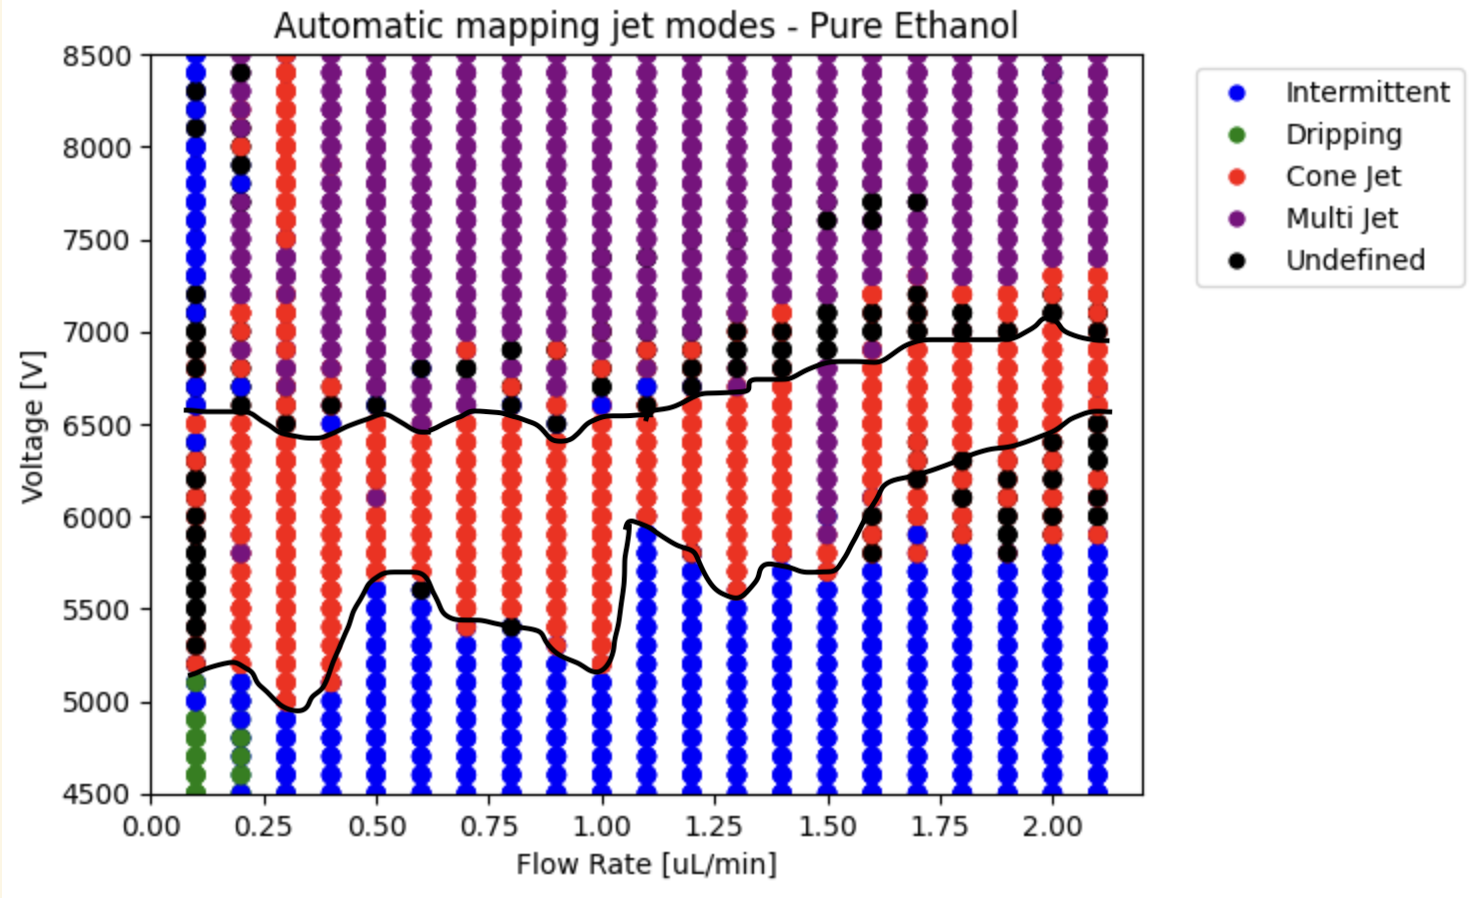
\includegraphics[width=9cm]{Figuras/report4/map7-automatic-line.png}
                \caption{ exp-26-01 automatic classification}
            \end{figure}


        \end{multicols}

        \subsection{Non-dimensional axis}

        To compare with the literature and validate the algorithm we decided to display the data using the non-dimensional numbers used in figure \ref{fig:ganan_calvo_fig}.

            \begin{figure}[H]
                \center
                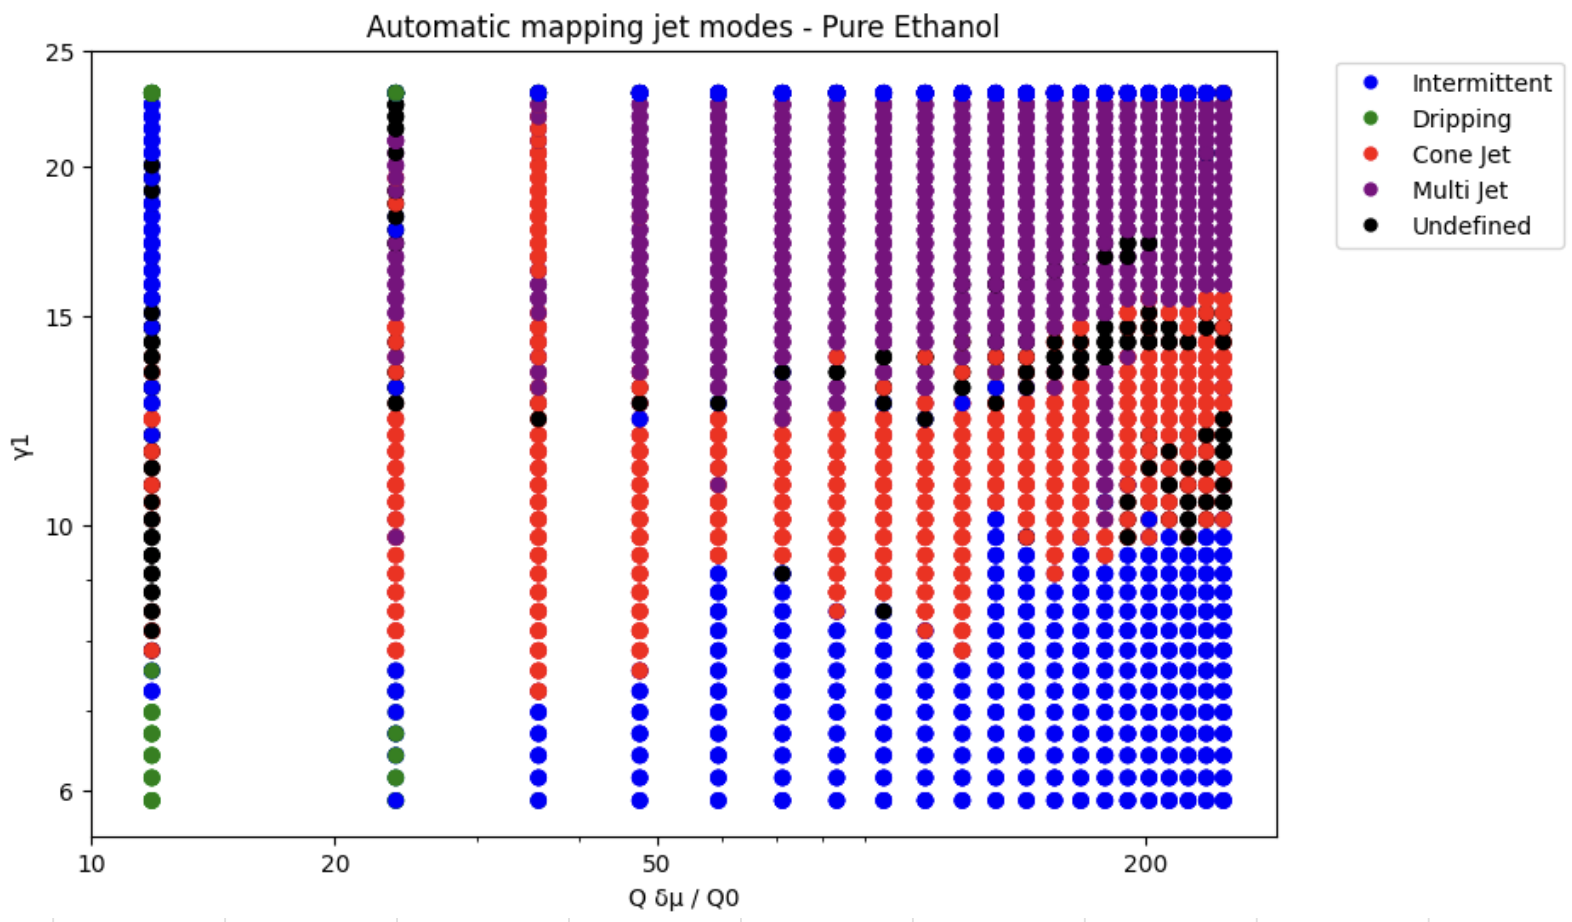
\includegraphics[width=12cm]{Figuras/19:03/non-dimensional-1.png}
                \caption{ exp-26-01-2 (V x Q)}
            \end{figure}

\section{Controller}
\label{sec:controller_results}


    \subsection{Simple Controller}

        \begin{algorithm}
            \caption{simple controller}\label{alg:simple_controller}
            \begin{algorithmic}
            \Function{controller}{$spray\_mode$} 
                
                \If{$spray\_mode$ = $'Intermittent'$ or $spray\_mode$ = $'Dripping'$}
                    \State \Call{send\_voltage\_command}{$voltage$ + 100}
                \ElsIf{$spray\_mode$ = $'Multi Jet'$ or $spray\_mode$ = $'Corona'$}
                    \State \Call{send\_voltage\_command}{$voltage$ - 100}
                \ElsIf{ $spray\_mode$ = $"Cone Jet"$}
                    \Comment{Keep Stable}
                \EndIf

            \EndFunction
            \end{algorithmic}
        \end{algorithm}

        Flowrate perturbation robustness test

        \begin{figure}[H]
            \center
            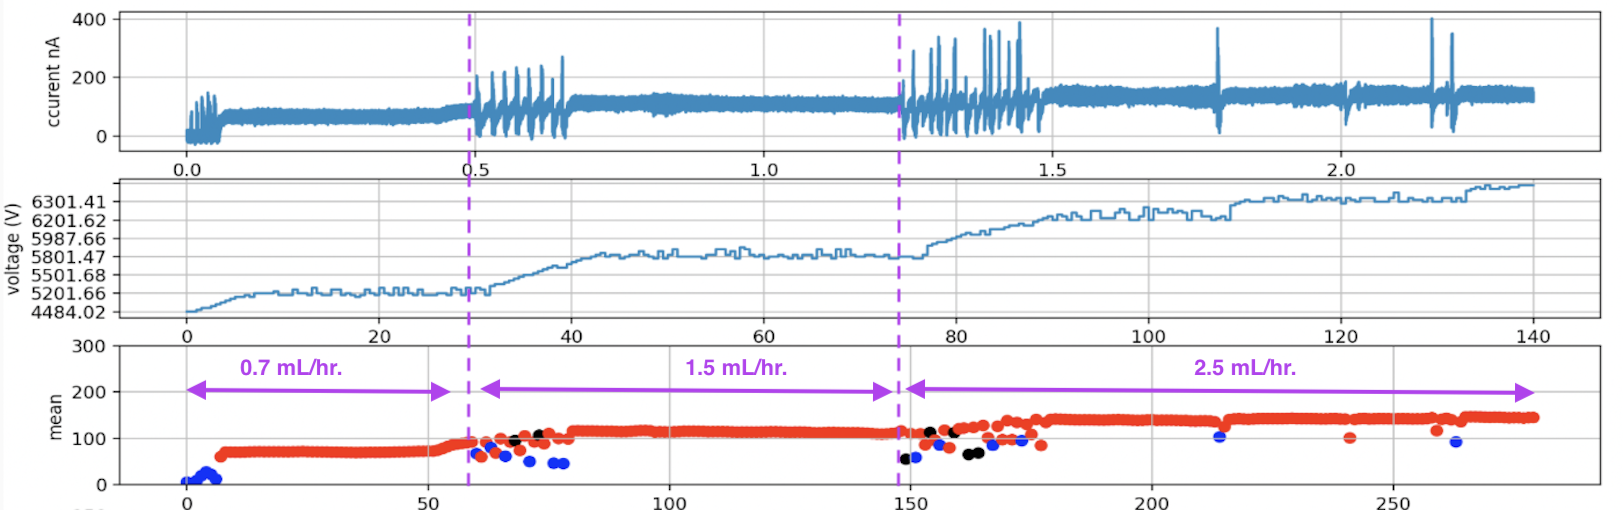
\includegraphics[width=15cm]{Figuras/19:03/control_first_results.png}
            \caption{ exp-26-01-2 (V x Q)}
        \end{figure}


    \subsection{Robust Controller}

    \subsection{Fuzzy Controller}

        The fuzzy approach of controller was explored and simulated but not used in the final version of the project.
        This because for this fuzzy approach we need to have the input variables for the fuzzy machine to be fuzzified.
        Which means that to use a fuzzy logic in our controller loop the classification must be fuzzyfied and our classification algorithm was not developed in order to give a classification and its current membership function.

        For that, I tried to fuzzyfi the controller input by the data acquired in the step routine. With the data I mapped the area of each spraying mode according to its potential and fuzzyfied this as shown in the Figure X.

        \begin{multicols}{2}
            \begin{figure}[H]
                \centering
                \resizebox{90mm}{!}{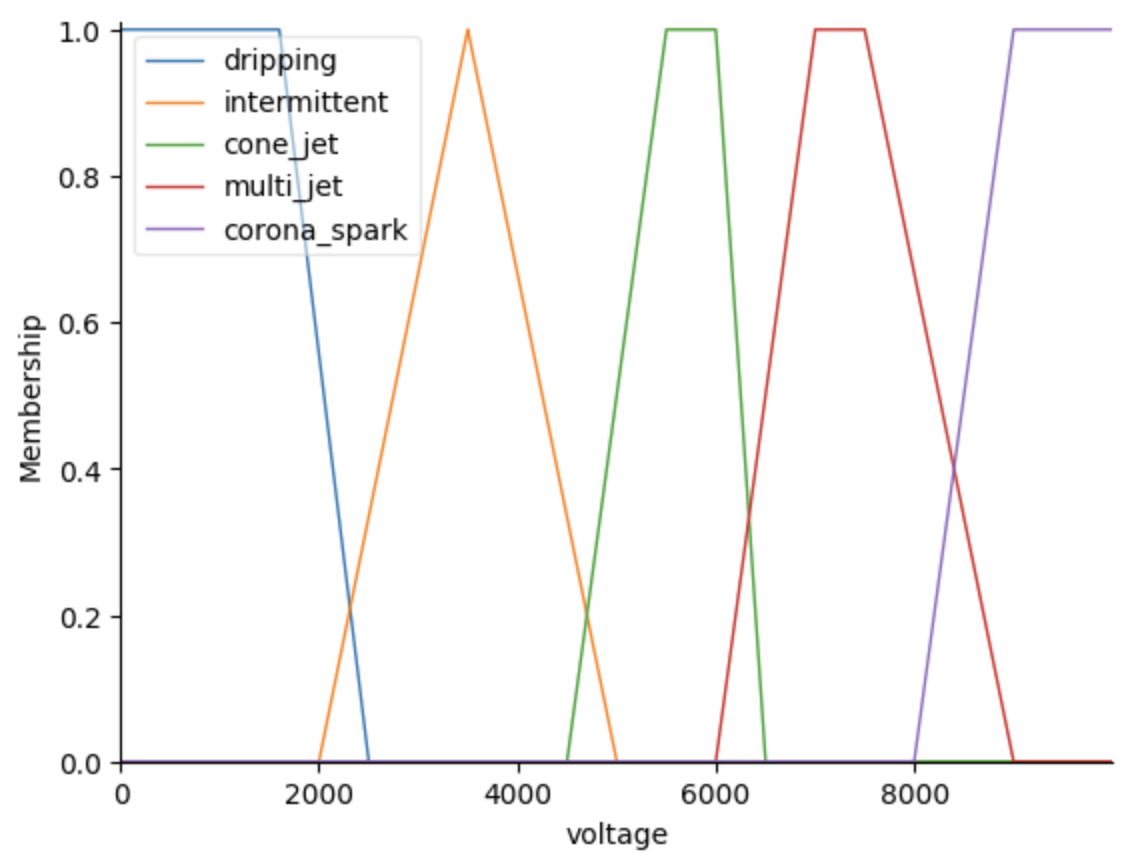
\includegraphics{Figuras/fuzzy/fuzzyfy_input.png}}
                \caption{Fuzzyfication}
                \label{fig:fuzzy_input}
            \end{figure}

            \begin{figure}[H]
                \centering
                \resizebox{90mm}{!}{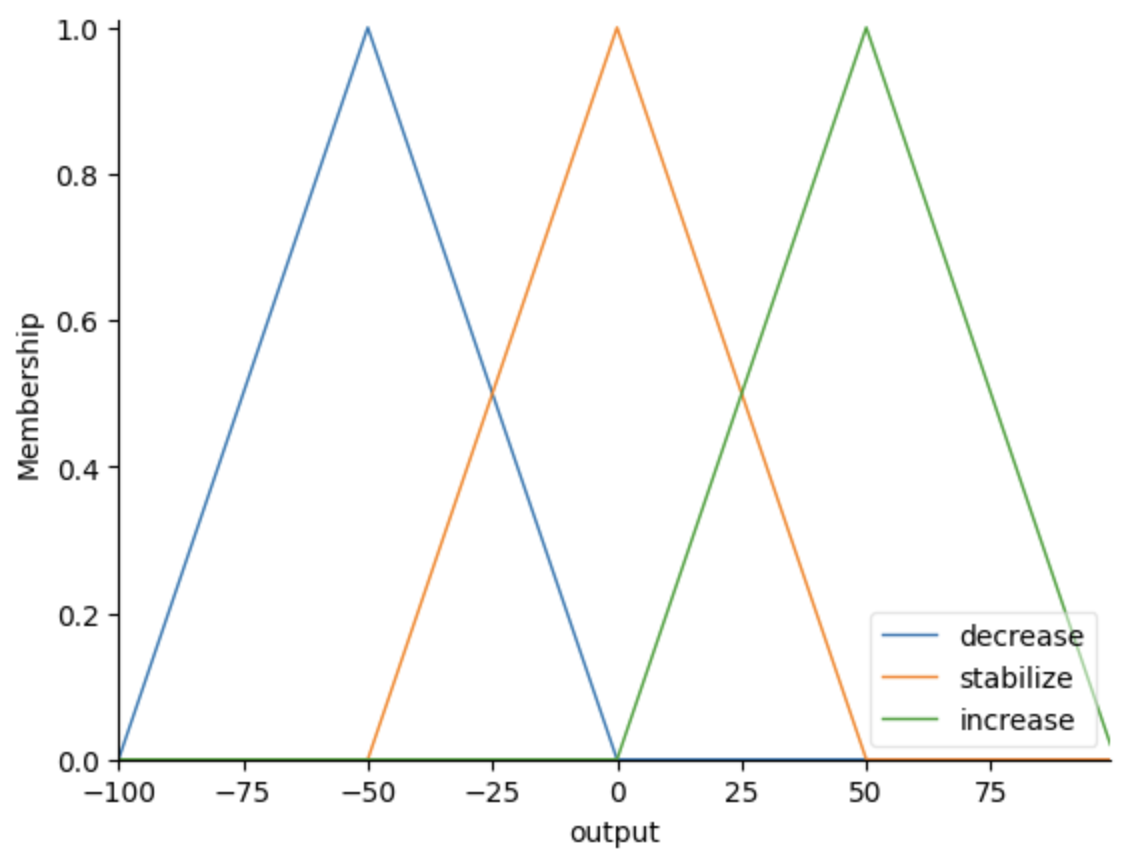
\includegraphics{Figuras/fuzzy/defuzzyfy.png}}
                \caption{Defuzzyfication}
                \label{fig:fuzzy_output}
            \end{figure}
        \end{multicols}

        \begin{figure}[H]
            \centering
            \resizebox{80mm}{!}{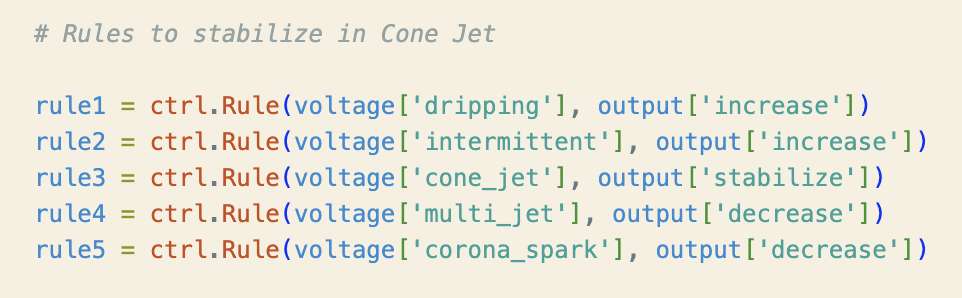
\includegraphics{Figuras/fuzzy/rules.png}}
            \caption{Fuzzy Rules}
            \label{fig:fuzzy_rules}
        \end{figure}

        \begin{multicols}{2}

            \begin{figure}[H]
                \centering
                \resizebox{90mm}{!}{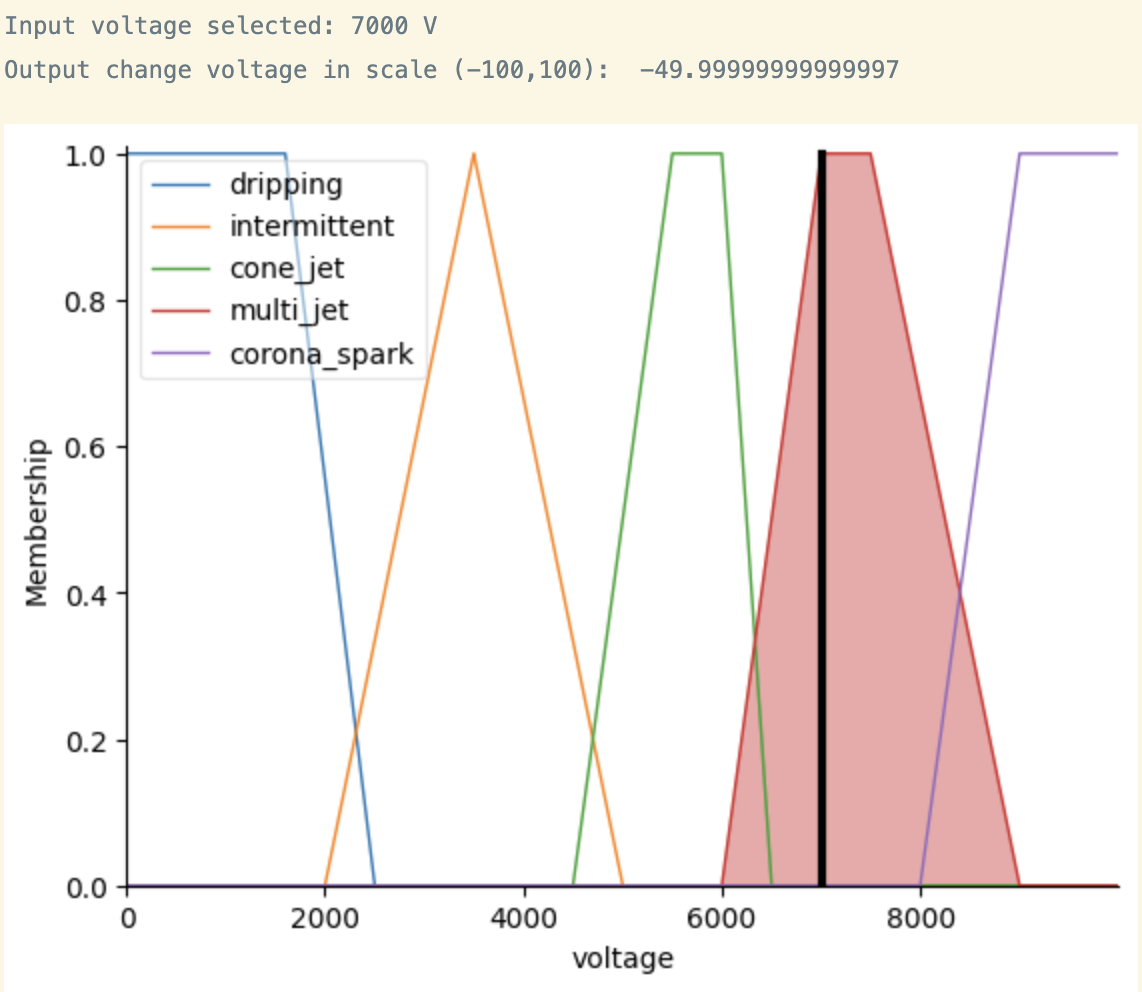
\includegraphics{Figuras/fuzzy/test1.png}}
                \caption{Test 1: fuzzy controller}
                \label{fig:fuzzy_test1}
            \end{figure}

            \begin{figure}[H]
                \centering
                \resizebox{90mm}{!}{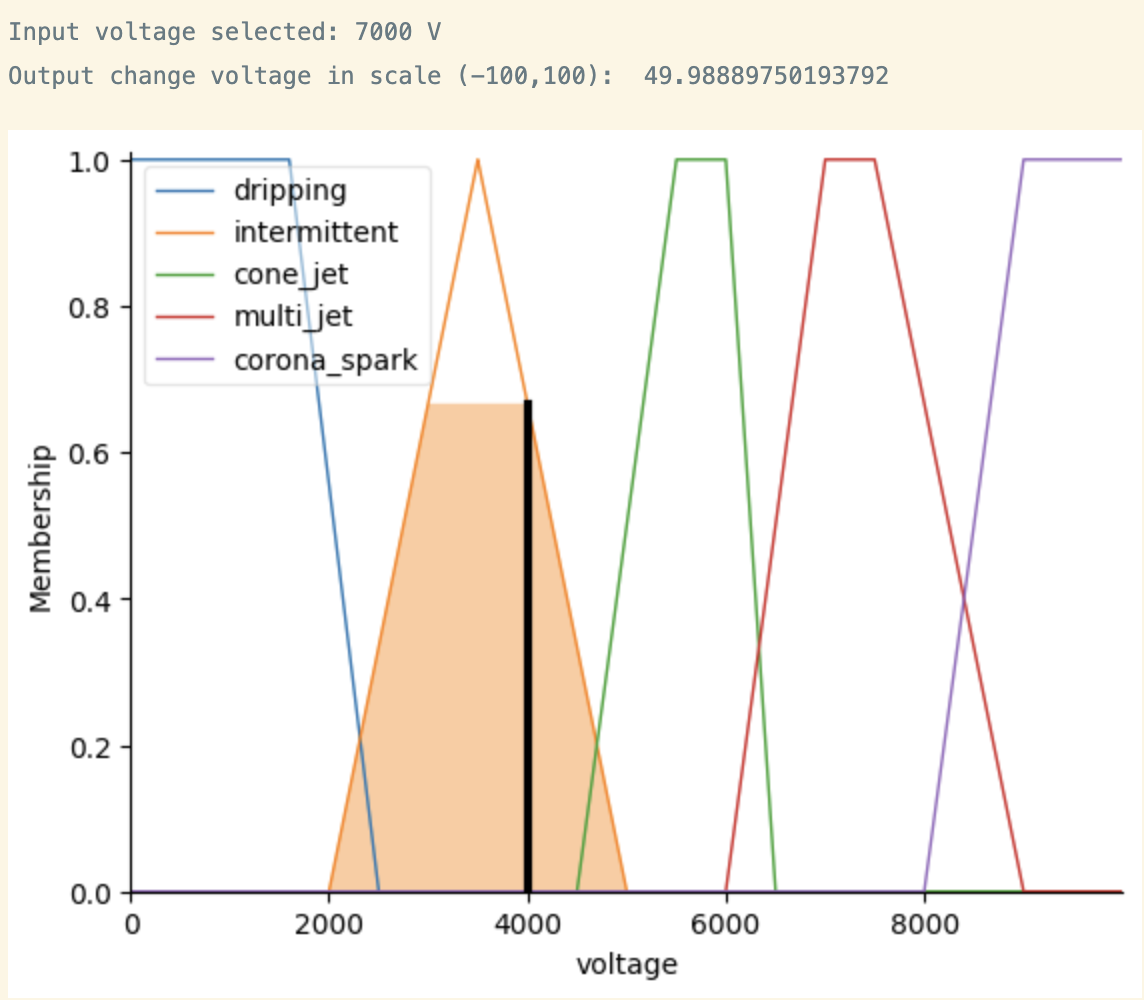
\includegraphics{Figuras/fuzzy/test2.png}}
                \caption{Test 2: fuzzy controller}
                \label{fig:fuzzy_test2}
            \end{figure}

        \end{multicols}


\clearpage